%\chapter{Further Perspectives for Monitoring the Software Process}

\chapter{Article 5: Software Process Evaluation from User Perceptions and Log Data}


{\bfseries \Large Authors: \medskip}

\noindent Damjan Vavpotič,
Saimir Bala,
Jan Mendling and,
Tomaž Hovelja \hfill

\bigskip

{\noindent\bfseries \Large Published in: \medskip}

\noindent Journal of Software: Evolution and Process

\bigskip

{\noindent\bfseries \Large Abstract: \medskip}


\noindent \textbf{Purpose} – Companies often claim to follow specific software development methodologies (SDM) when performing their software development process. These methodologies are often supported by dedicated tools that keep track of work activities carried out by developers. The purpose of this paper is to provide a novel approach that integrates analytical insights from both the perceptions of SDM stakeholders and software development tools logs to provide SDM improvement recommendations. \\

\noindent
\textbf{Design/methodology/approach} – This paper develops a new process improvement approach that combines two significantly different sources of data on the same phenomenon. First, it uses a questionnaire to gather software development stakeholder SDM perceptions (managers, developers). Second, it leverages process mining to analyse software development tools logs to obtain additional information on software development activities. Finally, it develops recommendations based on concurrent analysis of both sources. \\

\noindent
\textbf{Findings} – Our novel process improvement approach is evaluated in three directions: does the presented approach (RQ1) enable managers to gain additional insights into employees’ performance, (RQ2) deliver additional insights into project performance, and (RQ3) enable development of additional SDM improvement recommendations. We find that integrated analysis of software development perception data and software development tools logs opens new possibilities to more precisely identify and improve specific SDM elements.\\

\noindent
\textbf{Research limitations} – The evaluation of our novel process improvement approach follows a single case study design. Our approach can only be used in enterprises in which software development tools logs are available. The study should be repeated in different cultural settings. \\

\noindent
\textbf{Practical implications} – We practically show how concurrently analysing data about developer SDM perceptions and event log data from software development tools enables management to gain additional insights in the software development process regarding the performance of individual developers. \\

\noindent
\textbf{Originality/value} – The main theoretical contribution of our paper is a novel process improvement approach that effectively integrates data from management and developer perspectives and software development tools logs. \\

\noindent
\textbf{Keywords} – software development methodology, evaluation, stakeholder perceptions, software development tool logs, case study

\pagebreak


% Management/Monitoring Perspective and How these techniques contribute
% Trace data 

% 
%
%
%Make the title shorter.
%
%\todo[inline]{Polish the chapter}
%\todo[inline]{Decide with Jan what to do here. Keep/Kill?}
%\todo[inline]{Elaborate more on the text. Motivate this section by including the social science point of view. The previous chapters are belong more to software engineering.}

%The techniques presented in this dissertation fall under the broader category of analyses methods based on trace data. When used individually they provide specific insights about determinate perspective of a process. These methods can also be combined with one another in order to achieve a more complete picture about how the process performs under the different perspectives. Beyond measuring performance of processes, trace-data methods can be exploited in combination with other methods to aid theory development~\citep{DBLP:journals/isr/BerenteSS19}.
%
%This chapter presents two more approaches that leverage trace data to gather insights on the software development. \Cref{sec:combining-questionnaier-and-trace} explores a mixed-method approach to identify relevant software development elements. It combines a subjective perspective from questionnaires and data analyses from event logs. As a result, insights are gathered on what elements both considered important and are actually used. \Cref{sec:conversational-structure} presents an approach that leverages speech act theory to understand how conversation about software development unfold. As a result, it is possible to observe differences in the process of successful collaboration. 

%\chapter{Software development process evaluation based on integration of stakeholder perceptions and software development tool logs data}

\todo[inline]{Damjan work}

New important theoretical development for SDM evaluation - complementing stakeholder perceptions with data about actual execution of the software development process.

\section{What are the perceptions of developers and managers about the work?}

\section{What has been done in the past?}

\section{What we propose}

\section{Evaluation}

\section{Discussion}

\section{Introduction}


Software development methodologies (SDMs) highly influence the management of software projects. Adopting a specific methodology can determine to what extent performance goals such as cost, quality and timeliness are achieved \citep{DBLP:journals/bise/VavpoticRH20}.  Existing studies show \citep{kneuper2008cmmi,Loon2007,DBLP:conf/enase/LaporteOP15a} that the adoption of SDMs is critical for success of development teams, but not easy to apply in practice. More specifically, it is often the case that a specific methodology is either applied partially or incorrectly, is not suitable for the enterprise due to incompatible technical characteristics, or has unsatisfactory impact on software quality, cost and development time \citep{DBLP:journals/dss/ChanT09,balasubramanian2016evaluation}.  Therefore, understanding the performance of specific SDM elements is crucial for management’s capability to continuously improve software development processes \citep{DBLP:journals/comsis/VavpoticH12}. These SDM elements include SDM activities as well as artefacts produced and tools used in these activities. 


In order to gain knowledge of the current state of SDMs within software companies, newest approaches in literature have focused on the analyses of their constituting SDM elements  \citep{hovelja2015exploring,DBLP:journals/infsof/VavpoticB09,gill2018scaling}. These studies focus on perceptions of various stakeholders about software process activities, tools and roles and neglect software development process data from supporting tools. This additional source of information regarding development process became available in recent years with widespread use of tools used in software development activities like issue tracking, requirements management, test management etc. Such tools store valuable data about actual execution of the development process and can provide additional insights into SDM and its elements, thus complementing stakeholder perceptions \citep{DBLP:journals/ese/ChoetkiertikulD17,DBLP:conf/msr/MantylaADGO16,DBLP:journals/peerj-cs/DestefanisOCSMT16,DBLP:conf/icse/OrtuDKM15}. What these recent works do not address is to what extent both sources of information complement each other.


In this paper, we propose a novel approach to evaluate a process improvement approach of the performance of SDM activities through concurrent analysis of stakeholder perceptions and relevant software development tools logs. In this way, we can consider both sources of insights about performance of specific SDM activities and consequentially improve organisational learning \citep{annosi2020learning}. Based on this analysis we develop SDM improvement recommendations. We evaluated our approach through a case study in an Austrian SME software development company. 

This work seeks answers to the following research questions:

\begin{inparadesc}
	\item[RQ1.] Which new insights into employees’ performance for management does the proposed approach provide?
	
	\item[RQ2.] Which new insights into project performance for management does the proposed approach provide?
	
	\item[RQ3.] Which new insights does the concurrent analysis of stakeholder SDM perception data and software development logs provide and which SDM improvement recommendations would be otherwise unavailable?
	 
\end{inparadesc}


The rest of the paper is organized as follows. Section 2 provides background on the state of the art. Section 3 describes the methodology. Section 4 applies the methodology on a case study from industry and shows the results. Section 5 discusses the results and their implications. Section 6 concludes the paper.

\section{State of the Art}

This paper builds upon existing research on \glsfirst{sdm} evaluation and process mining. In the following, we briefly introduce these fields of research. 

\subsection{SDM evaluation}
\label{subsec:sdm-sota}

Existing research shows that using SDMs improves productivity of software development enterprises and quality of the developed software \citep{DBLP:journals/infsof/Bass16,DBLP:journals/re/ZdravkovicSG15,DBLP:journals/access/TuapeHKPK21}. This is achieved by increasing enterprises’ ability to transfer knowledge between employees, systematically manage software development process, etc. \citep{avison2006information,DBLP:journals/iam/Fitzgerald98,hovelja2015exploring,DBLP:journals/tse/RiemenschneiderHD02}. However, it is not enough that an enterprise only describes its SDM in a document; the developers need to use it consistently in their everyday work. The use of SDM was often a topic of research in the last decades, since SDM adoption among software developers was relatively low and the developers often preferred different ad hoc approaches \citep{DBLP:journals/software/Aaen03,DBLP:journals/isj/Fitzgerald96,DBLP:journals/iam/HuismanI06}. According to \cite{DBLP:journals/peerj-cs/DestefanisOCSMT16} developers are the key factors for the success of a software development process, not merely
as executors of tasks, but as protagonists and core of the whole development process. Therefore,
understanding their perceptions is of key importance in SDM improvement.

The use of SDMs in enterprises can be analysed with the help of different approaches based on Technology Acceptance Model, Theory of Planned Behaviour, etc. \citep{aboelmaged2010predicting,venkatesh2000theoretical,DBLP:journals/behaviourIT/WangLH13}. One of the foundational theories in the field of SDM evaluation is diffusion of innovations \citep{DBLP:books/daglib/0012785}, according to which SDM is considered as innovation that developers adopt \citep{DBLP:journals/iam/Gallivan03,DBLP:journals/infsof/GreenHC05,Huisman2002}. To obtain information about the studied SDM and its elements the aforementioned studies focused on SDM perceptions held by different stakeholders, namely developers, managers, users, etc. to measure characteristics like level of use, assimilation, social and technical suitability, developer satisfaction and impact on performance \citep{atkinson1999project,cooper1990information,DBLP:books/daglib/0012785,DBLP:journals/infsof/VavpoticB09,DBLP:journals/comsis/VavpoticH12,DBLP:journals/infsof/HodaNM11}. By considering opinions of multiple
stakeholders our approach fits well with agile SDM that emphasize team autonomy, decentralized
decision making, flexible scope and managing a high degree of requirement changes \citep{DBLP:journals/smr/ScottMKP21,DBLP:journals/software/Jorgensen19}.


Detailed insight into SDM and its elements can be gained by comparing the perceptions of different stakeholders regarding the same SDM and/or its element \citep{hovelja2015exploring}. 
Another important theoretical development in the field was that SDM should be studied at the level of its constituent elements like activities, tools, roles, produced documents, etc. and not only as a whole. This improved the understanding of suitability of studied SDM elements for a certain development team and enabled comparison between the studied SDM elements; thus, allowing enterprises to better pinpoint problematic elements of SDM, prepare focused improvements and examine the link between a specific SDM element and overall project success \citep{atkinson1999project,hovelja2015exploring}. Such development is in line with findings in the field of situational method engineering \citep{DBLP:journals/ejis/KarlssonA09,DBLP:conf/caise/RalyteDR03,gill2018scaling,Malinova2022} that constructs a custom SDM from those SDM elements that fit with characteristics of certain development team and other situational factors (internal and external enterprise’s environment).
One of the key goals of these improvements was to tackle low SDM
adoption rates which process and practice improvement initiatives often suffer from \citep{DBLP:conf/profes/FontdevilaGOP19}. Such low adoption rates clearly indicate the inadequacy of existing SDM evaluation models and the need to develop better ones, for instance based on the analysis of log data.

\subsection{Analysis of Event Logs}
\label{subsec:data-an-sota}

Process mining is a discipline that gained popularity in the last decade. The goal of process mining is to provide fact-based insights and support process improvement. On a broader context, process mining can be considered as the missing link between traditional model-based process analysis and data driven techniques such as data mining and machine learning. Van der Aalst \citep{DBLP:books/sp/Aalst16}, defines four partially overlapping perspectives of a business process that are widely used in business process modelling (BPM) community. First, the \emph{time perspective} aims at analyzing time and frequency of process events. Second, the \emph{case perspective} aims at identifying properties of process cases. Third, the \emph{organizational perspective} aims at analyzing the event log to gain transparency on the resources involved in the process. Fourth, the \emph{control-flow perspective} aims at analyzing the different variations of the process, i.e., in which order its constituting activities are carried out in real life. These aspects can be, for example, related to the control flow (i.e., the various steps used by the company for generating value), resources (i.e., handover of work among the different process participants), activities (i.e., how the work is broken down into several tasks), and data (i.e., which artifacts are produced and consumed by the process). 

Process mining is becoming widely adopted. While researchers can use general purpose data-mining tools like R, Orange, IBM SPSS, etc., a considerable number of specialized tools such as Celonis\footnote{https://www.celonis.com}, Disco\footnote{https://fluxicon.com/disco}, Apromore\footnote{https://apromore.org}, minit\footnote{https://www.minit.io}, LANA Process Mining\footnote{https://lanalabs.com/en}, etc. have been developed. A comparison of the current process mining tools can in found in \cite{viner2021process}. In academia, log analysis is an established endeavor when it comes to gaining insights into software development. Recent works
\citep{DBLP:conf/wecwis/MarquesSF18,DBLP:conf/bpm/BalaCMRP15,DBLP:conf/bpm/BalaRGBMS17,Bala2018b,DBLP:conf/ifip8-1/BalaKM20} demonstrate potential for understanding the different perspectives of processes. Process mining has also been considered as a research method \citep{DBLP:conf/hicss/GrisoldWMB20}  with applications for analyzing process improvement methods \citep{DBLP:conf/hicss/GrossMM19} and reporting software experiments \citep{DBLP:journals/ese/RevoredoDM21}.

Continuous evolution of data analyses techniques (such as process mining), their adoption in new domains and their integration into other research methods in different mixed-methods approaches, indicate the future opportunities that novel SDM evaluation approaches can exploit. In this context, the necessity and importance of our research that attempts to integrate current state of the art process mining approaches and SDM evaluation approaches becomes clear, since the integration can deliver insights that neither of the two approaches alone can provide.

\section{Proposed Approach}


\subsection{Overview}

In this section, we present our novel process improvement approach. The development of our
approach followed principles from design science \citep{Hevner2004}  and
situational method engineering \citep{DBLP:books/sp/Henderson-SellersRAR14} as research
methods. The proposed approach builds on the established SDM evaluation approaches. \Citet{gill2018scaling} emphasize the need for project to meet stakeholders’ expectations thus analysis of different
stakeholders’ perceptions must be an integral part of a modern SDM evaluation approach. \Citet{DBLP:journals/infsof/VavpoticB09} showed the importance of evaluating SDMs by their constituent parts and not only
as a whole. \Citet{DBLP:journals/comsis/VavpoticH12} presented the usefulness of considering economic success
metrics of software development in SDM evaluation. However, unlike existing approaches that base
their SDM evaluation solely on stakeholder perceptions, the proposed approach complements
stakeholder perceptions with data from software development tools logs. The approach comprises
four phases as shown in \Cref{fig:sdm-approach}. To our knowledge, this is the first attempt to combine perceptions
and log data in SDM evaluation. Next, we elaborate on the phases of the approach.


%The proposed approach builds on the established SDM evaluation approaches \citep{gill2018scaling,DBLP:journals/infsof/VavpoticB09,DBLP:journals/comsis/VavpoticH12}. However, unlike existing approaches that base their SDM evaluation solely on stakeholder perceptions, the proposed approach complements stakeholder perceptions with data from development tools’ event logs. The approach comprises four phases as shown in \Cref{fig:sdm-approach}. 

\begin{figure}
	\centering
	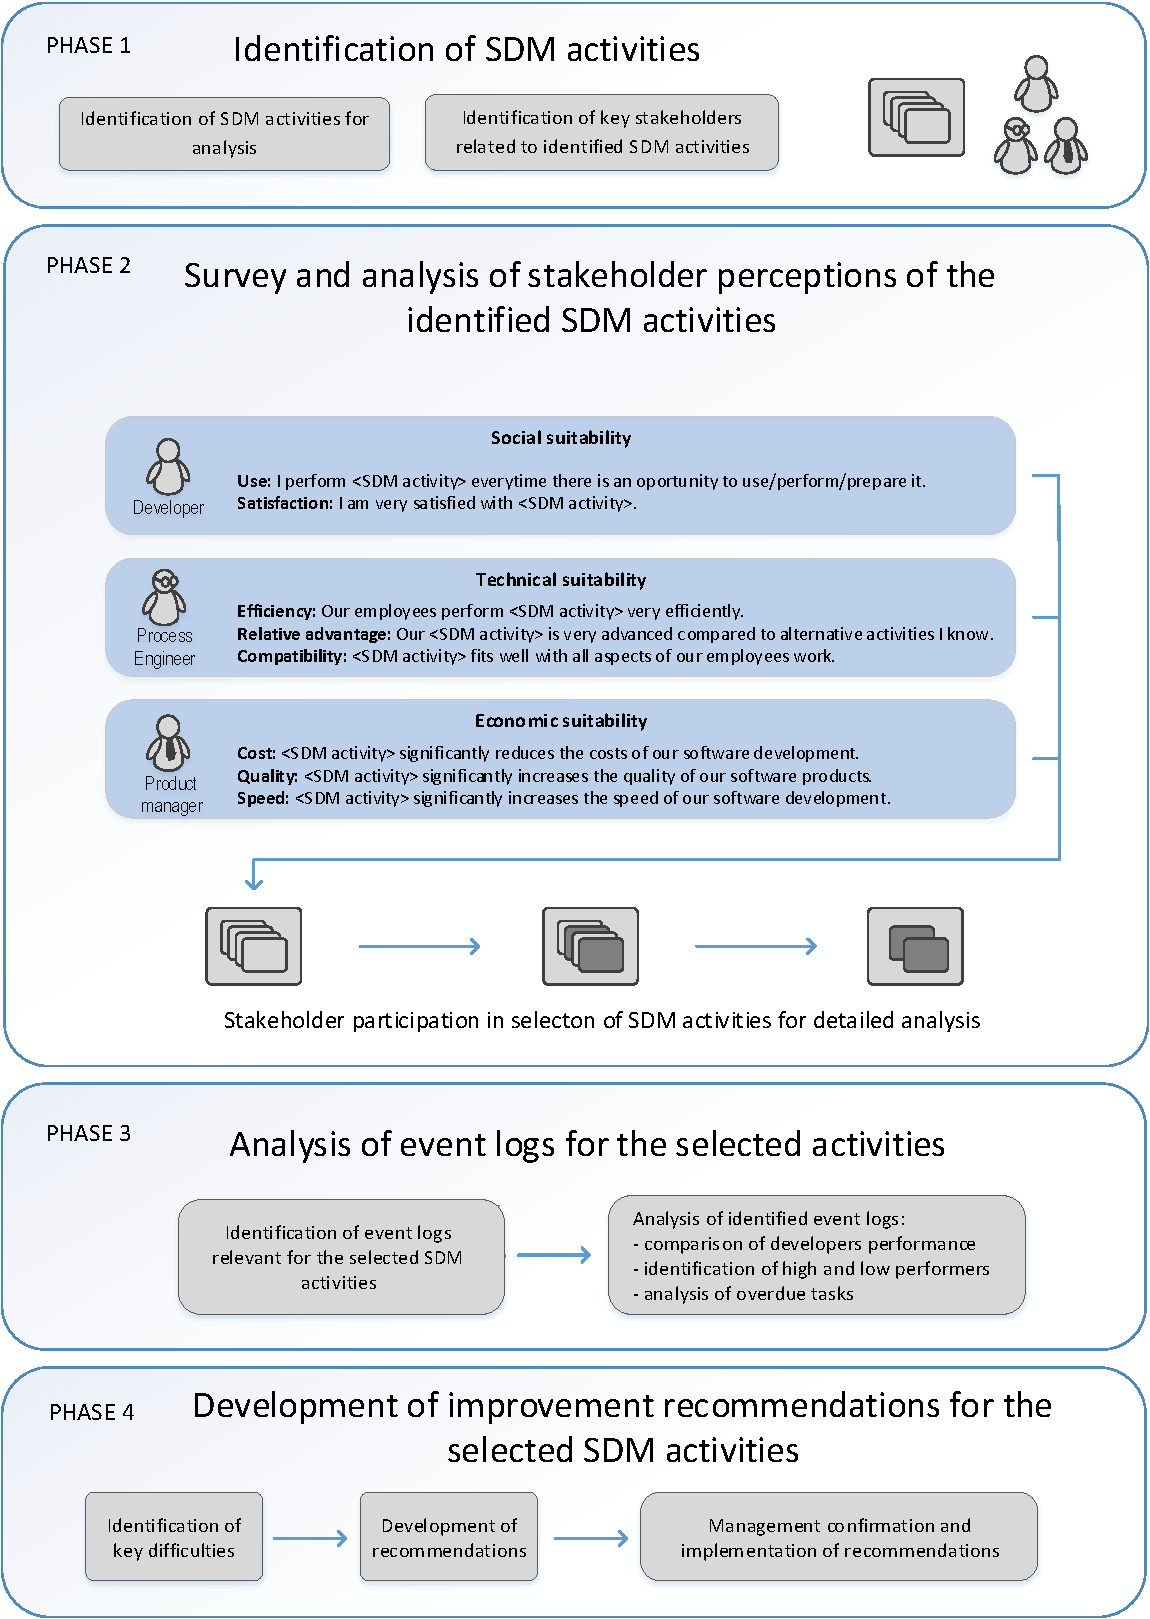
\includegraphics[width=\linewidth]{figures/sdm-latest}
	\caption{The proposed SDM evaluation approach}
	\label{fig:sdm-approach}
\end{figure}


\subsection{Phase 1 – Identification of SDM Activities}

In Phase 1, SDM activities for evaluation are first identified and catalogued with the help of
key stakeholders knowledgeable about their SDM (e.g., lead developers, managers). In identification
phase we focus on activities since log data are typically organized around them. Roles are considered
indirectly as specific activities are typically performed by a specific role. If an enterprise formally
follows a specific standard SDM (like Scrum, IBM Rational Unified Process, Kanban, etc.), the
cataloguing starts with a predefined list of typical SDM activities. However, the key stakeholders still
have to point out which SDM activities are actually used and identify possible additional activities in
the enterprise and only those are included in the final catalogue. After the SDM activities are
catalogued the management has to identify the actual stakeholders performing these activities in a
specific project that will be evaluated. Managers responsible for a certain project and/or product
should be the ones to evaluate the SDM activities used in project and/or product development from
managerial perspective. Similar logic is also applied to other project stakeholders.

\subsection{Phase 2 – Survey and analysis}
Phase 2 starts with the creation of questionnaires that include each SDM activity catalogued
in Phase 1 based on the template questions (shown in Fig. 1). Different questionnaires are created
for each stakeholder. In line with the established measures from studies presented in the literature
review the developers evaluate SDM activity social suitability (average of use and satisfaction).
Similarly, product managers evaluate SDM impact on iron triangle measures of economic suitability
(average of cost reduction, speed increase and quality increase). The questions are written in form of
statements where answers are given on 7-point Likert scale.

To analyse stakeholder perceptions, we position SDM activities in a multidimensional space
where each dimension represents a specific stakeholder perspective. It is typically difficult to further
improve SDM activities that are considered highly beneficial by all stakeholders since they are all already satisfied with them. On the contrary, SDM activities that are considered unbeneficial by all
stakeholders have high potential for improvement, since it is likely that most stakeholders will
support their change. The SDM activities where perceptions of stakeholders are very low and/or
greatly differ require further examination where log analysis (Phase 3) has an important role to
identify appropriate improvement actions.


\subsection{Phase 3 – Analysis of software development tools logs for selected activities}

In Phase 3, log analysis is performed focusing on selected SDM activities. Log analysis
provides additional information about certain SDM activities such as the time developers spent their
execution of this activity and the quality of the execution. To guide the log analysis, we followed the
\pmsquare methodology \citep{DBLP:conf/caise/EckLLA15}. \pmsquare consists of six stages, namely
(1) planning – in which the goals and the target processes are identified, (2) extraction – in which trace data
of the identified processes are collected, (3) data processing – in which data is transformed into
event logs, (4) mining \& analysis – in which the event logs are analysed by means of process mining
techniques, (5) evaluation – in which results of process mining are interpreted and linked to
improvements ideas, and (6) process improvement \& support – in which the improvement ideas are
implemented.

When it comes to analysing SDMs, \pmsquare can be adapted as follows. First (1), we start the log
analysis with identification of software development tools logs relevant for the selected SDM
activities. Second (2), event logs are gathered from the respective information systems. Then an
inspection of the information contained in these logs is performed to confirm that relevant
information about resources and activities is present. Third (3), data processing is performed. In fact,
different software development tools have their own logging mechanisms and often use customized
representations of event logs. Such logs are rarely in the format needed by process mining tools.
Therefore, pre-processing is required in order to transform these logs into a format which can be further analysed by process mining techniques \citep{DBLP:journals/tkde/AalstWM04,DBLP:conf/bpm/LeemansFA14}. Therefore, the data is stored into a form of a flat table with explicitly
labelled notions of case, activity and timestamp. This representation can be easily transformed into
the standard XES~\citep{verbeek2010xes} format for event logs or be
directly consumed process mining tools.

Fifth (5), we analyse instances of activities preformed during development that are described
by at least three aspects: activity type (bug fixing, implementing new code, etc.), actor (employee
ID1, employee ID2, etc.), and timestamp (date1, date2, etc.). These three aspects enable us to
analyse identified software development tools logs to compare developers’ performance, identify
high and low performers and analyse overdue activity instances for specific types. To conduct these
analyses depending on log structure different process mining techniques can be used like analyses of
case durations, filtering on users, variant analyses. Moreover, some software development tools logs
contain additional information like priority of specific types of activities, pointers to related or
preceding activities, detailed unstructured descriptions of preformed activities and comments, etc. If
needed, these can be used to gain additional insights into the software development process as a
whole as well as into specific SDM activities \citep{Hamdy2020}. As we focus on a single case, we
use process mining to support exploring these different aspects related to the selected SDM
elements.

Finally (5 \& 6), several analyses artifacts resulting from the applications of the
aforementioned process mining techniques such as process maps, case/activity/user frequency
reports and durations of activities are collected. For instance, for the SDM element of bug-fixing, we
can observe how often this was worked on by a certain user and whether it took the user one or
more sprints to complete his task. These kinds of insights are then compared to the perceptions
collected via the questionnaire to help resolving conflicting perceptions. For instance, it may the case
that management does not perceive correctly the time and effort spent by developers on bugs.Equipped with evidence-based results from event logs, it is possible to align the perceptions of the
different stakeholders.


\subsection{Phase 4 – SDM improvement recommendations}
In this phase, systematic and comprehensive data from Phase 2 and 3 is presented to external and/or internal SDM experts (if enterprise has sufficient competences). Their task is to identify key difficulties of the current development process based on the concurrent analysis of stakeholders SDM perceptions and software development tools logs. Next, based on identified key difficulties they prepare recommendations for process improvement using their knowledge and experience. Different problem-solving techniques like brainstorming, simulation, what-if-analysis, creativity techniques, etc. that help to support the act of improving can be used in this phase. An example of recommendations developed by such approach is presented in Case study section. Finally, the recommendations need to be presented, discussed with and confirmed by the management. After management acceptance of the proposed recommendations a timeline for their implementation can be developed. 

\section{Case Study}

\subsection{Case study description and research methodology}
The proposed approach was tested in an Austrian SME software development company located in Vienna. The company can be considered a typical central European SME. The company develops a software platform in the field document composition, workflow and document distribution. Their customers come from eight different central and southern European countries. Seven developers and a product manager worked on company’s customer communications management (CCM) platform in the studied year. The product manager oversaw the quality of the product features, software process speed and cost. All developers participating in our study were experienced developers having worked as members of the same team for at least two years.

The company uses Scrum \citep{takeuchi1986new} an agile, lightweight, iterative and incremental methodology often used in software development. Scrum organizes work in iterations called sprints. The length of sprint is set in advance and is typically between one week and one month, with two weeks being the most common. As in most Scrum implementations each sprint starts with sprint planning and ends with sprint review (presenting work to stakeholders) and sprint retrospective (identifying issues and improvements related to the development process). 

The company uses the JIRA issue tracking software to monitor tasks completion by their developers. We obtained data for two activities (implementing new code, bug fixing) from 26 sprints for 5 developers working on the studied activities between 2016-01-11 and 2017-01-08. The JIRA event log was pre-processed to generate a flat table. In tabular datasets, we created additional attributes to track the number of performed activities. We aggregated the information into two-week intervals reflecting company sprints. This helped us understand if the studied activities were completed on schedule (in one sprint) or not. Furthermore, JIRA allows us to track activity completion rate on the level of the whole project and on the level of individual developers. 

An exploratory case study design was employed to assess the proposed approach \citep{DBLP:journals/ese/RunesonH09}. Such design is appropriate when it captures the circumstances and conditions of an everyday or commonplace situation \citep{yin2009case}. The studied company represents a typical SME in the software development industry. To collect the data, we conducted interviews with management, directly observed their workday, surveyed all developers working on the observed project and collected the corresponding JIRA event logs. The study results were presented and validated by the SME’s management.

\subsection{Identification of SDM activities (Phase 1)}
In the first phase, we identified ten key activities (\Cref{tab:identified-activities}) of the company’s software development process by interviewing the lead developer and product manager.  They also specified the other developers who worked on this project. The identified ten activities cover key parts of the SDM used in the company. These include requirements specification, planning, coding with unit testing and maintenance. We also identified JIRA logs that were used in one or more of the identified ten activities in the observed period.

% Please add the following required packages to your document preamble:
% \usepackage{booktabs}
% \usepackage{graphicx}
\begin{table}[]
\centering
\caption{Identified activities and availability of JIRA logs}
\label{tab:identified-activities}
\resizebox{\textwidth}{!}{%
\begin{tabular}{@{}lcl@{}}
\toprule
Development activities                         & Availability of JIRA logs related to the activity &  \\ \midrule
Defining 				list of specifications (in Excel) & No                                                &  \\
Defining 				feature specifications            & Yes                                               &  \\
Using 				prepared feature specification       & Yes                                               &  \\
Using 				prepared bug specification in Jira   & Yes                                               &  \\
Estimating 				(planning poker)                & No                                                &  \\
Assigning 				from Backlog to sprint           & No                                                &  \\
Implementing 				new code                      & Yes                                               &  \\
Bug 				fixing                                 & Yes                                               &  \\
Sprint 				planning  (bi-weekly)               & Yes                                               &  \\
Stand-ups 				(Daily meetings)                 & No                                                &  \\ \bottomrule
\end{tabular}%
}
\end{table}

\subsection{Survey and analysis of stakeholder perceptions of the identified SDM activities (Phase 2)}
\label{subsec:phase2}

Based on the template questions (Fig. 1) we created two separate questionnaires, one for the seven developers and one for the product manager. For the purpose of the analysis, we visualize the results of the survey of the two identified stakeholders on a scatter chart comprising the developers’ perspective as a horizontal dimension and the product manager’s perspective as a vertical dimension (\Cref{fig:survey-scatter-plot}).

\begin{figure}
	\centering
	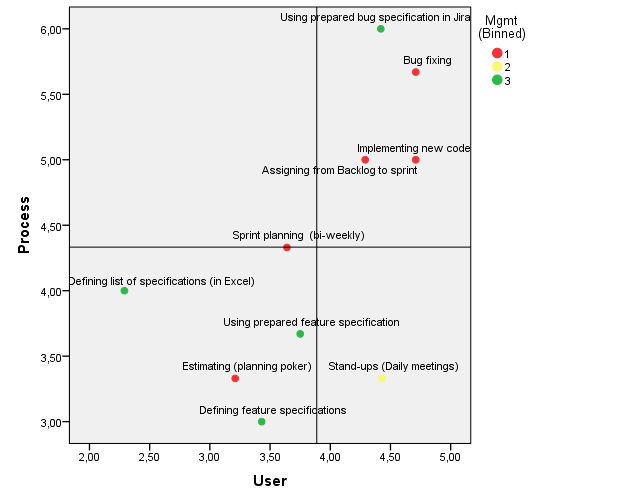
\includegraphics[width=\linewidth]{figures/survey-scatter-plot}
	\caption{Scatter chart of stakeholder views on the identified development activities}
	\label{fig:survey-scatter-plot}
\end{figure}


To better understand the views of the two stakeholders on specific SDM activities four quadrants were formed in the scatter chart by using the average scores of developers’ and management perspectives. The four quadrants follow the logic suggested by \cite{DBLP:journals/comsis/VavpoticH12}: the first quadrant contains managerially and socially unsuitable SDM activities, the second quadrant contains managerially unsuitable but socially suitable SDM activities, the third quadrant contains managerially suitable but socially unsuitable SDM activities and the fourth quarter contains managerially and socially suitable SDM activities. Each SDM activity is presented by a point in one of the four quadrants of the scatter chart. The red colour points represent the five activities that were selected for detailed evaluation. Management limited the selection of activities for analysis and improvement to maximum half of all SDM activities (i.e. five activities) due to limited capabilities and resources available for the improvement processes. The selection was done as follows. All SDM activities that were unbeneficial for both stakeholders (Sprint planning and Estimating) were selected for further analysis from the first quadrant (I). From the second quadrant (II) the two SDM activities (Implementing new code and Bug fixing) that consume significantly more work hours per sprint were selected. While from the third quadrant (III) one SDM activity was selected (Defining list of specifications) that was significantly lower graded by the developers.

User stories described in \emph{Defining feature specifications} activity were prioritized and assigned to a list (backlog) in \emph{Defining list of specification} activity. During the interviews we learned that that the main reason for dissatisfaction of developers with \emph{Defining list of specification} activity was that management was often adjusting prioritizations of user stories to ensure customer satisfaction when customer priorities changed. Due to regular shifts in customers’ priorities, this approach caused difficulties for developers who often had to de-prioritize user stories related to architecture and other technical aspects. The dissatisfaction of the developers was further exacerbated by the fact that they felt team autonomy and team ability to plan its work was affected. Moreover, the list of specifications was maintained in MS Excel, which caused additional difficulties for the developers due to delayed list synchronization. 

The \emph{Estimating (planning poker)} and \emph{Sprint planning (bi-weekly)} activities were performed by the team each sprint as follows. First, the team performed \emph{Estimating (planning poker)} to determine the effort needed for each task. Next, in \emph{Sprint planning (bi-weekly)} these tasks were divided among the team members. According to the management, these activities were among the least efficient activities. The management was dissatisfied by often exceeded time limits as tasks were not completed in a single sprint as planned. The dissatisfaction of the team was mostly the result of increased but unsuccessful management pressure to raise performance.

\emph{Implementing new code} and \emph{Bug fixing} activities were time-wise the main activates in the development process. While the developers were satisfied with their performance, seeing themselves as highly capable performers and valuable employees, the management did not share their view and considered these two activities similarly inefficient as \emph{Estimating (planning poker)} and \emph{Sprint planning (bi-weekly)}. The main cause of management dissatisfaction was again poor compliance with task completion time limits set by the team.

\subsection{Analysis of event logs (Phase 3)}
\label{subsec:phase3}

We analyzed JIRA logs related to four out of the six selected development activities with available JIRA logs to gain new insights especially where the views of management and developers differed. \emph{Defining list of specification} was maintained in MS Excel, thus no JIRA logs were available. First, we analyzed the frequency of bugs and tasks not completed in each examined sprint (26 sprints = 1 year) to get additional insights in \emph{Estimating (planning poker)} and \emph{Sprint planning (bi-weekly)} activities. \Cref{fig:frequency-of-bugs} shows the number of not completed bugs per sprint and Figure 4 shows the number of not completed tasks per sprint. In both cases, there is considerable variability in unfinished tasks/bugs between sprints. This exposes planning and performance difficulties as well as an unstable development process. 


\begin{figure}
	\centering
	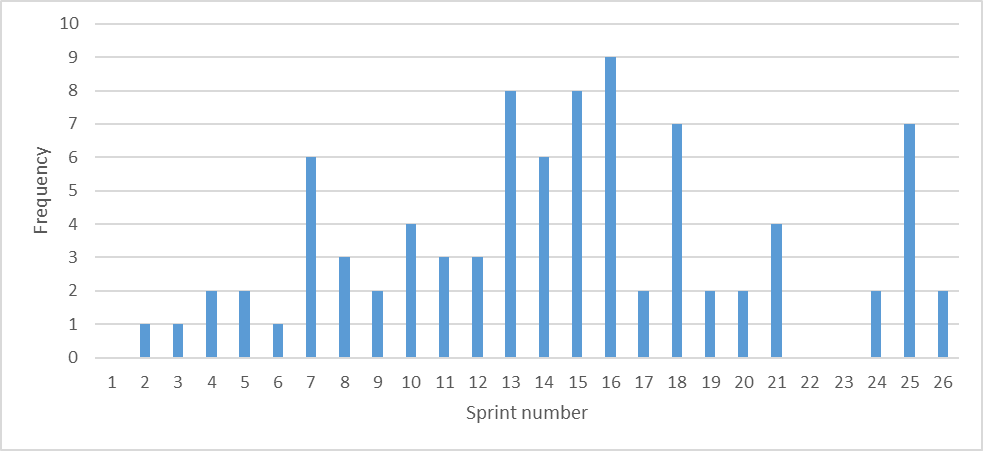
\includegraphics[width=\linewidth]{figures/frequency-of-bugs}
	\caption{Frequency of bugs not completed in a single sprint by sprint number}
	\label{fig:frequency-of-bugs}
\end{figure}

\begin{figure}
	\centering
	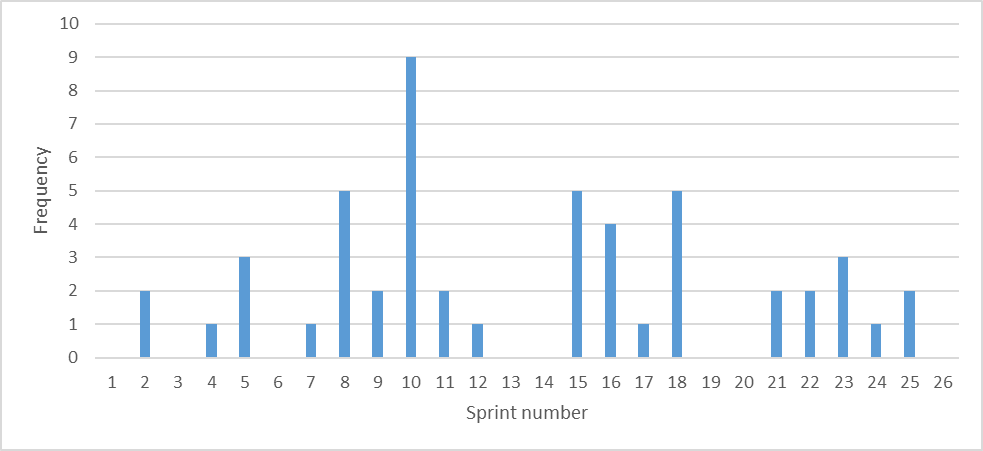
\includegraphics[width=\linewidth]{figures/frequency-of-tasks}
	\caption{Frequency of tasks not completed in a single sprint by sprint number}
	\label{fig:frequency-of-tasks}
\end{figure}


To gain additional insights in \emph{Bug fixing} and \emph{Implementing new code} activities we compiled \Cref{tab:bug-and-tasks-completed}. It shows the individual developer performance breakdown in number and percentage of bugs fixed and new code implementations (tasks completed) in a single sprint and those completed in more than one sprint. 

% Please add the following required packages to your document preamble:
% \usepackage{booktabs}
% \usepackage{multirow}
% \usepackage{graphicx}
\begin{table}[]
\centering
\caption{Bugs and tasks completed in a single sprint and in more than one sprint for each developer\\
* = Developer 1 was performing only Bug fixing (bugs), while the other four developers were performing Implementation of new code (tasks) and Bug fixing.}
\label{tab:bug-and-tasks-completed}
\resizebox{\textwidth}{!}{%
\begin{tabular}{@{}llllllll@{}}
\toprule
\multicolumn{2}{l}{}                                                      & Developer 			1 & Developer 			2 & Developer 			3 & Developer 			4 & Developer 			5 & Total  \\ \midrule
\multirow{3}{*}{Number 			of bugs}  & Completed 			in a single sprint      & 22     & 22     & 17     & 39     & 30     & 130    \\
                                    & Completed 			in more than one sprint & 12     & 16     & 17     & 33     & 9      & 87     \\
                                    & Total                                & 34     & 38     & 34     & 72     & 39     & 217    \\
\multirow{2}{*}{Percentage 			of bugs}  & Completed 			in a single sprint & 64,7\%         & 57,9\%         & 50,0\%         & 54,2\%         & 76,9\%         & 59,9\% \\
                                    & Completed 			in more than one sprint & 35,3\% & 42,1\% & 50,0\% & 45,8\% & 23,1\% & 40,1\% \\
\multirow{3}{*}{Number 			of tasks} & Completed 			in a single sprint      & *      & 78     & 18     & 16     & 19     & 131    \\
                                    & Completed 			in more than one sprint & *      & 10     & 15     & 8      & 18     & 51     \\
                                    & Total                                & *      & 88     & 33     & 24     & 37     & 182    \\
\multirow{2}{*}{Percentage 			of tasks} & Completed 			in a single sprint & *              & 88,6\%         & 54,5\%         & 66,7\%         & 51,4\%         & 72,0\% \\
                                    & Completed 			in more than one sprint & *      & 11,4\% & 45,5\% & 33,3\% & 48,6\% & 28,0\% \\ \bottomrule
\end{tabular}%
}
\end{table}

The analysis of performance clearly shows significant differences between individual developers. Additionally, there were significant differences in on-time completion rate between \emph{Bug fixing} and\emph{ Implementation of new code}, showing that if a developer is a top performer in one activity he can still struggle in the other. The most extreme cases were Developer 2 and Developer 5. On one hand, Developer 2 was the best performer in \emph{Implementation of new code}, but was below average in \emph{Bug fixing}. On the other hand, Developer 5 was the best performer in \emph{Bug fixing}, but the worst in \emph{Implementation of new code}. Developers 3 and 4 were below average in both activities. Additionally, Developer 3 was relatively worse in \emph{Implementing new code}. Developer 1 was above average in Bug fixing, however he did not participate in \emph{Implementing new cod}e.

This information derived from log analysis allowed us to gain the following additional insights for the four selected development elements with available JIRA event logs.

The logs show that there is significant variability in task and bugs completion rates between developers, thus the management perception that developers’ performance was not satisfactory was only partially correct. JIRA event logs helped us determine that there are some great performers, some average performers and some poor performers.  To tackle this problem successfully, these differences have to be better managed in order to improve \emph{Estimating (planning poker)} and \emph{Sprint planning (bi-weekly)} activities. If this issue is properly addressed, management can also expect improvements in \emph{Implementing new code} and \emph{Bug fixing} activities.

\subsection{Development of improvement recommendations for selected SDM activities (phase 4)}

Based on the above presented analysis in Phases 2 (\cref{subsec:phase2}) and 3 (\cref{subsec:phase3}) of the proposed approach, the following improvement recommendations were prepared for implementation by management (see \Cref{tab:key-difficulties}). 

% Please add the following required packages to your document preamble:
% \usepackage{booktabs}
% \usepackage{graphicx}
% \usepackage[normalem]{ulem}
% \useunder{\uline}{\ul}{}
\begin{table}[]
\centering
\caption{Identified key difficulties and SDM improvement recommendations }
\label{tab:key-difficulties}
\resizebox{\textwidth}{!}{%
\begin{tabular}{@{}m{1cm}m{3cm}m{1cm}m{6cm}@{}}
\toprule
 &
  Identified key difficulties &
   &
  SDM improvement recommendations \\ \midrule
D1 &
  Adjusting prioritizations of user stories to ensure customer satisfaction when customer priorities changed &
  R1 &
  Currently manager is acting as an intermediary 			between developers and the customer. Management needs to start to 			act as connector that encourages and helps the team to establish 			direct collaborations between them and the customer’s product 			owners (lead users). This would increase the team’s autonomy and 			ability to plan its work and at the same time enable the team to 			better consider the architectural and other technical aspects when 			prioritizing user stories. \\ \\ \hdashline \\
D2 &
  Delayed synchronization of list of specifications in MS Excel &
  R2 &
  The list of specifications that is currently 			managed in MS Excel should be moved to JIRA. This will integrate 			backlog with task planning and task completion administration. \\ \\ \hdashline \\
D3 &
  Unsuccessful management pressure to raise performance &
  R3 &
  Instead of pressure to stop undesirable behaviour we suggest management focuses on rewarding desirable 			behaviour. Thus, we suggest to revamp the reward scheme and make a 			desired but still achievable percentage of tasks/bugs completed in 			time an important metric of remuneration. \\ \\ \hdashline \\
D4 &
  Often exceeded estimated sprint tasks time limits in implementing new code and bug fixing &
  R4 &
  To address this difficulty, we propose using individual developer performance data mined from JIRA logs to 			increase the efficiency of task distribution between the 			developers. The developers who are significantly more efficient at 			bug fixing should predominantly work on bug fixing, while the 			developers who are significantly more efficient at implementing 			new code should predominantly work on new code. Additionally, the 			first, the second and the third improvement also partially address 			this difficulty. \\ \bottomrule
\end{tabular}%
}
\end{table}

\subsection{Reflection workshop with company management}

The identified difficulties and prepared recommendations were presented and discussed with the company management in order to assess their validity and usefulness. The management provided feedback as follows:

\begin{itemize}
	\item The management strongly agreed with the first identified difficulty and the recommendation of the experts to give developers more autonomy and direct contact to the customer. They modified their requirements acquisition process so that it was performed by dedicated team members and not by the management.
	
	\item The management strongly agreed with the second identified difficulty and followed the recommendation to move the list of specifications to JIRA. This simplified the development process and reduced the process quality issues.
	
	\item The management strongly agreed with the third identified difficulty, but only partially followed the third recommendation. They did lessen the pressure on the developers but did not change the remuneration by linking it to performance. To lessen the pressure, they organized a yearly meet-up with core customers where developers themselves could estimate the time needed for development of requested features.  This prevented the management to overpromise and overcommit to the core customers.
	
	\item The management strongly agreed with the fourth identified difficulty and followed the recommendation by providing the relevant performance data mined from JIRA event logs about the efficiency of task distribution between the developers to the team to improve their sprint planning.
	
	\item Management confirmed that this is a novel approach, and they could not specify any other similar approach. Existing SDM approaches (Scrum, Kanban, etc.) do not use process mining to evaluate SDM elements. 
	
	\item Management confirmed that the proposed approach was useful and relevant in the context of SDM.
	
\end{itemize}
	
Overall, we found that management not only agreed with the identified difficulties but also found the results highly relevant to improve their process. As they stressed in the interview, despite the rich set of features provided by current supporting tools such as JIRA, there is still an unmet need for a higher-level integrated reporting process which can give better insights on the overall status of the SDM. 


\section{Discussion}

\subsection{Addressing research questions}

We successfully addressed the three research questions posed in the paper and found that the proposed approach enables managers to gain additional insights into employees’ performance (RQ1), since the information from software development tools logs allows for an improved performance management of individual developers by knowing their exact on time sprint task/bug completion rates (\Cref{tab:bug-and-tasks-completed}). Next, we confirmed that the proposed approach delivers additional insights into project performance through monitoring the frequency of total tasks/bugs not completed in a single sprint (RQ2). Finally, we ascertained that the concurrent analysis of software development perception data and software development tools logs enables additional SDM improvement recommendations (RQ3). 

The first and second recommendation (R1 and R2 in \Cref{tab:key-difficulties}) are based on perception analysis alone since log analysis does neither help us identify the first two key difficulties (D1 and D2 in \Cref{tab:key-difficulties}) as important software development issues nor it can be used to improve the two recommendations (R1 and R2). However, the development of the third and fourth recommendations (R3 and R4 in \Cref{tab:key-difficulties}) would not be possible without the concurrent analysis of perception and log data.  R3 and R4 require software development tools logs to provide exact sprint task and bugs completion rates needed for improved individual developer performance management, while the perceptions provide the context about managers’ satisfaction with specific performance levels.

\subsection{Contribution}

Our case study showed several theoretical and practical implications of the proposed approach. The main theoretical contribution of our paper is a novel approach for evaluation of performance of SDM activities through concurrent analysis of stakeholder (managers and developers) perceptions and relevant software development tools logs. Its contribution is not primarily in specifying how managers and experts should develop insights and recommendations, but to present how combined sources of information (software development tools logs and perception data) will allow them to develop better recommendations and gain insights that otherwise would not be achievable. The approach combines the state of the art from the field of SDM evaluation (presented in \Cref{subsec:sdm-sota}) and the field of log data analysis (presented in \Cref{subsec:data-an-sota}) that were previously not connected. We hope that establishing this bridge enriches both fields and contributes to their further development.

We practically demonstrated how software development tools logs enable management to gain additional insights in the software development process regarding the performance of individual developers. Additionally, we showed how software development tools logs could be used to monitor the performance of an agile team by tracking the percentage and number of unfinished tasks after each sprint. It is important to know that these findings can only be gained by concurrently analysing subjective qualitative SDM perceptions of developers and management, and quantitative software development tools logs data which importantly complement each other. On one hand, focusing only on log data lacks stakeholder context and is thus often difficult or even impossible to contextually correctly interpret. On the other hand, focusing only on stakeholder SDM perceptions can often lack important details that allow management to gain deeper understanding of specific issues since perceptions are typically collected on a more general level. 

Management response that confirmed the validity of the proposed approach was added to the discussion. To ensure construct validity we used multiple sources of information including surveys and interviews with key stakeholders, log data and confirmation of the results with management. Internal validity was confirmed through two activities. The first activity was careful analysis of stakeholder perception and software development tools logs where we did not identify any conflicting information. The second activity was addressing rival explanations with management, which showed consistency between our interpretation and management views.  This indicates strong consistency and internal validity of information and explanation.  A typical central European software development SME using agile SDM was selected for the case study to ensure representative results and as much external reliability as possible. We believe that the approach can be scaled up and also be used in non-agile settings, however it was only tested in an agile SME setting. To ensure reliability use case study protocol was carefully followed \citep{yin2009case}.	


\subsection{Threats to validity and other limitations}

Four important limitations need to be considered. Firstly, there are limitations of external validity, namely generalization. At this stage we were able to conduct only a single case study in an agile setting. Although, we picked an Austrian SME that is representative for SMEs in the IT sector in central Europe, additional case studies in multiple settings would help confirm the broader usefulness of the approach as well as strengthen its theoretical and practical implications. Secondly, the approach can only be used in enterprises in which software development tool logs are available. Thirdly, the study should be repeated in different cultural settings to see if other cultural contexts would importantly affect the usefulness of the approach. Lastly, due to variability of software development tools logs it is not possible to define a universal step-by-step procedure for analysis of software development tools logs, however this is often the case in the field of process mining.

Similarly, as other approaches in the field of process improvement \citep{Zellner2011} our approach does not specify a step-by-step procedure with the aim to replace experts and managers and their ability to interpret data and develop recommendations. On the contrary, it empowers experts and managers with new information based on concurrent analysis. Moreover, it is impossible to formalize a procedure that would produce appropriate recommendation for each and every company since the context of companies can differ greatly. Thus, experts and managers need to be employed to interpret the information provided by our approach and produce the final insights and recommendations. 


\section{Conclusion}

The main contribution of the study is a novel approach for evaluation of software development process that concurrently considers stakeholder SDM perceptions and data from software development tools logs. In a case study, we confirmed the effectiveness of the proposed approach and identified its theoretical and practical contributions to the studied field. We successfully addressed the three research questions posed in the paper and discussed its validity and limitations. 

Future work should expand the number of case studies in different cultural settings and test different sources of log data that would enable measuring not only developer performance, but also process and product quality. Furthermore, in the field of SDM perception analysis additional stakeholders should be considered (business partners, customers, etc.). Finally, as the field of process mining is rapidly evolving new methods and tools should be considered. Current automation trends in software development field generate ever increasing number of software development tools logs which will offer future researchers an opportunity to perform more comprehensive long-term analyses. 


%\chapter{The Conversational Structure of Problem-Solution Co-Evolution}

\section{First section}

